\documentclass{beamer}

\usepackage[utf8]{inputenc}
\usepackage[ngerman]{babel}
\usepackage{beamerthemeshadow}
\usepackage{calc}
\usepackage{ifthen}
\usepackage{tikz}
\usepackage{caption}
\usepackage{subcaption}
\usepackage{bchart}
\usepackage{wrapfig}
\usepackage{ulem}
\usepackage{color}
\usepackage{epigraph}
\usepackage{tipa}
\usepackage{hyperref}
\usepackage{url}
\usepackage{amsmath}

\setbeamertemplate{caption}[numbered]

\usepackage[
	european,
	europeanvoltages,
	europeanresistors,
	europeanports
	]{circuitikz}

% \usepackage{pgf-pie}

\definecolor{darkgreen}{rgb}{0.2,0.6,0.2}

\usepackage{listings}

\title{Kollaboratives Texten}
\subtitle{Analyse und Portrait des FOSA-Projektes}
\author{Ervin Mazlagi\'c, Daniel Winz}
\institute{FOSA}

\begin{document}
%\thispagestyle{empty}
\maketitle

\section{Einleitung}

\subsection{Person}
\begin{frame}
	\frametitle{Wer sind wir? \hfill{} \footnotesize{FOSA}}
	\begin{block}{Ervin Mazlagi\'c 
		\hfill{} 
		\footnotesize{Core Developer}}
		\begin{itemize}
			\item Elektroniker, HW-Entwicklung
			\item FreeSoftware, LuXeria
			\item ET-Studium HSLU
		\end{itemize}
	\end{block}
	\vfill{}
	\begin{block}{Daniel Winz
		\hfill{}
		\footnotesize{Founder, Core Developer}}
		\begin{itemize}
			\item Elektroniker, HW-Entwicklung
			\item Modellfliegen, LuXeria
			\item ET-Studium HSLU
		\end{itemize}
    	\end{block}
\end{frame}

\subsection{Ziele}
\begin{frame}
	\frametitle{Was wollen wir erreichen? \hfill{} \footnotesize{FOSA}}
	\begin{exampleblock}{Wir möchten, dass Sie wissen \dots}
		\begin{itemize}
			\item was FOSA ist und macht
			\item wie sich FOSA organisiert und arbeitet
			\item welche Beziehung Sie zur FOSA haben
		\end{itemize}
	\end{exampleblock}
	\vfill{}
	\begin{alertblock}{Wir möchten \textbf{nicht} \dots}
		\begin{itemize}
			\item auf technische Details eingehen
			\item jeden Gast zur Mitarbeit überzeugen
			\item unsere Produkte anwerben
		\end{itemize}
	\end{alertblock}
\end{frame}

\subsection{Programm}
\begin{frame}
    \frametitle{Programmübersicht \hfill{} \footnotesize{FOSA}}
    \tableofcontents[hideallsubsections]
\end{frame}

\section{FOSA}

\subsection{Idee und Ziele}
\begin{frame}
	\frametitle{Was ist FOSA? \hfill{} \footnotesize{FOSA}}
	\begin{block}{FOSA ist \dots mittlerweile der Name für vieles!}
		\begin{itemize}
			\item eine Gruppe bei Github
			\item ein Projekt von Studenten
			\item einige Formelsammlungen 
		\end{itemize}
	\end{block}
\end{frame}

\begin{frame}
	\frametitle{Wie ist FOSA entstanden? \hfill{} \footnotesize{FOSA}}
	\begin{block}{Meilensteine der Entwicklung}
		\begin{itemize}
			\item Erste Notizen als \LaTeX~Code
			\item Portierung auf Github
			\item Erweiterung des Core-Development Teams
			\item Entstehung eigener IT-Infrastruktur
			\item Build-Server und Webdienst online
			\item Erste Print-Ausgaben
		\end{itemize}
	\end{block}
\end{frame}

\begin{frame}
	\frametitle{Wer macht bei FOSA mit? \hfill{} \footnotesize{FOSA}}
	\textit{"`Gerade dann, wenn man am wenigsten freie Zeit hat, 
	macht man in der Tat am meisten."'}

	\hfill{} --- (Nino Ninux)
	\vfill{}
	\begin{block}{Core-Team}
		\begin{itemize}
			\item Core-Developer
				\begin{itemize}
					\item Daniel Winz 
						\hfill{} \footnotesize
						ET, BB \normalsize
					\item Ervin Mazlagi\'c
						\hfill{} \footnotesize
						ET, BB \normalsize
				\end{itemize}
			\item Maintainer
				\begin{itemize}
					\item Adrian Imboden
						\hfill{} \footnotesize
						INF, BB \normalsize
				\end{itemize}
		\end{itemize}
	\end{block}
\end{frame}

\begin{frame}
	\frametitle{Wer macht bei FOSA mit? \hfill{} \footnotesize{FOSA}}
	\framesubtitle{Graphische Analyse von Github --- fosamath}
	\begin{figure}
		\centering
		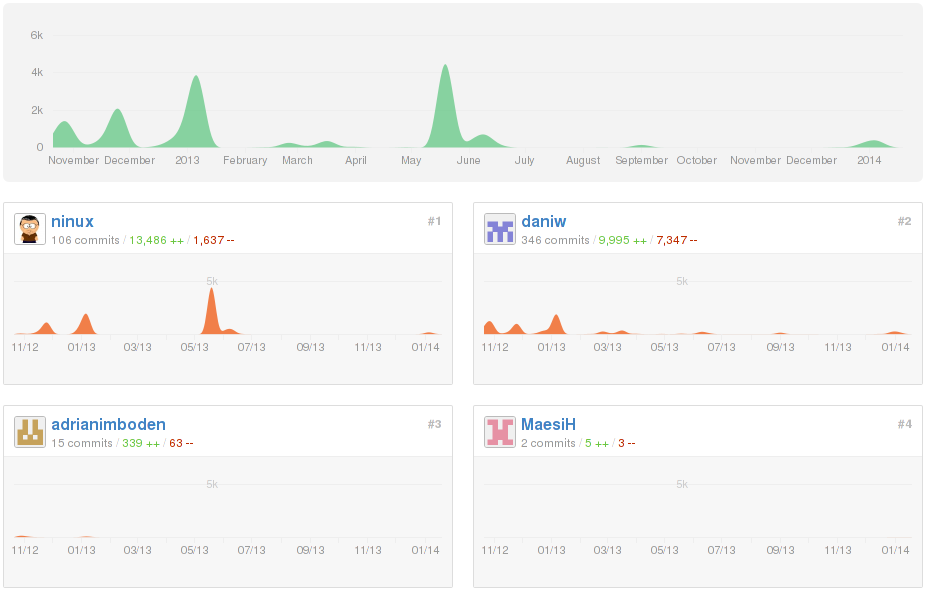
\includegraphics[width=0.9\textwidth]{fig/fosamath-additions.png}
	\end{figure}
\end{frame}

\begin{frame}
	\frametitle{Wann arbeitet man bei FOSA mit? \hfill{} \footnotesize{FOSA}}
	\framesubtitle{\dots meistens dann, wenn man keine Zeit hat!}
	\begin{figure}
		\centering
		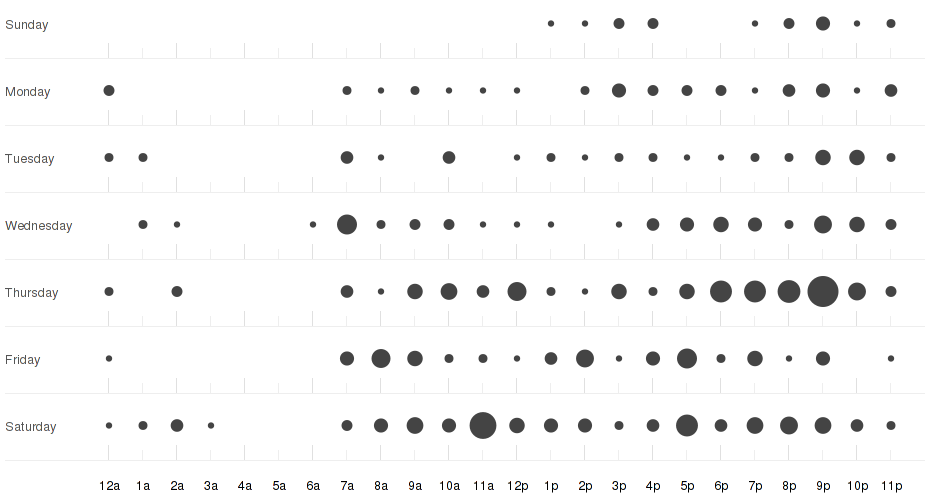
\includegraphics[width=1\textwidth]{fig/fosamath-punchcard.png}
	\end{figure}
\end{frame}

\begin{frame}
	\frametitle{Wozu eigentlich FOSA? \hfill{} \footnotesize{FOSA}}
	Wir möchten eine \textbf{freie} Sammlung von 
	Formelbüchern erstellen, welche auf die Inhalte der HSLU-T\&A
	abgestimmt sind.
	\vfill{}
	\begin{exampleblock}{Die vier Freiheiten 
		\hfill{} 
		\footnotesize{R. Stallman}}
		\begin{itemize}
			\item[F0] freies Benutzen des Originals 
				\hfill{} \footnotesize{"`run"'}
				\normalsize
			\item[F1] freies Teilen des Originals
				\hfill{} \footnotesize{"`redistribute"'}
				\normalsize
			\item[F2] freies Anpassen 
				\hfill{} \footnotesize{"`change"'}
				\normalsize
			\item[F3] freies Teilen des Geänderten 
				\hfill{} \footnotesize{"`release"'}
				\normalsize
		\end{itemize}
	\end{exampleblock}
\end{frame}

\begin{frame}
	\frametitle{Wieso ist uns FreeSoftware wichtig? 
		\hfill{} 
		\footnotesize{FOSA}}
	\textit{"`Freiheit wird in der Regel verstanden als die 
	Möglichkeit, ohne Zwang zwischen verschiedenen Möglichkeiten 
	auswählen und entscheiden zu können."'} 
	
	\hfill{} --- (Wikipedia)
	\vfill{}
	\textbf{Alles was obige Definition oder die vier Freiheiten
	verletzt, ist für uns schlicht keine Option!}
	\vfill{}
	\begin{exampleblock}{Unsere Freiheiten sind unantastbar dank \dots}
		\begin{itemize}
			\item Free Software 
				\hfill{} 
				\footnotesize{Tools, Formate}
				\normalsize
			\item General Public License (Copyleft) 
				\hfill{}
				\footnotesize{gpl-violations.org}
				\normalsize
		\end{itemize}
	\end{exampleblock}
\end{frame}

\subsection{Organisation}
\begin{frame}
	\frametitle{Wie arbeitet FOSA zusammen? 
		\hfill{} \footnotesize{FOSA}}
	\begin{block}{Hohe Kohäsion und lose Kopplung!}
		\begin{itemize}
			\item \TeX, \LaTeX 
				\hfill{} 
				\footnotesize{D. E. Knuth, L. Lamport} 
				\normalsize
			\item git -- "`the stupid content tracker"'
				\hfill{}
				\footnotesize{L. Torvalds}
				\normalsize
			\item github -- Social Coding
			\item Jenkins -- Continuous Integration
				\hfill{}
				\footnotesize{java}
				\normalsize
		\end{itemize}
	\end{block}
\end{frame}

\begin{frame}
	\frametitle{Der FOSA-Kreislauf}
	\begin{figure}
		\centering
		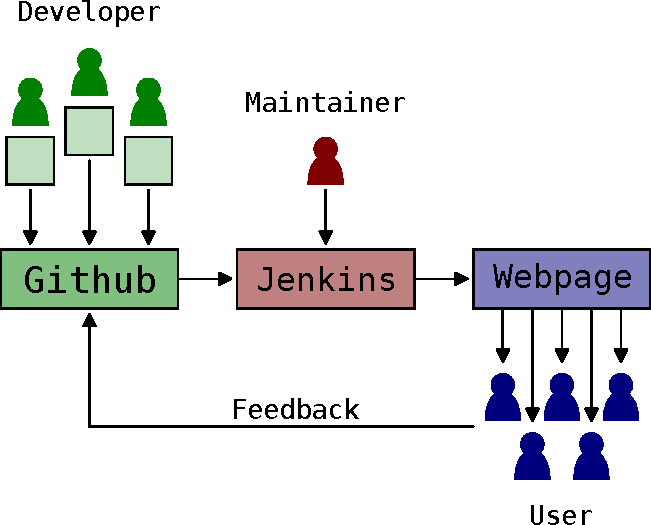
\includegraphics[width=0.7\textwidth]{fig/fosa-loop.pdf}

	\end{figure}
\end{frame}

\subsection{Tools}
\begin{frame}
	\frametitle{Was ist \TeX~und \LaTeX?}
	\begin{columns}
		\begin{column}{5cm}
			\TeX~ ist sowohl eine Programmiersprache als auch 
			ein Programm welches \dots
			\begin{itemize}
				\item von D. E. Knuth stammt
				\item gemacht wurde um Bücher zu schreiben
				\item Autoren Inhalte und Layout trennen 
					lässt
				\item Lesbaren Code zu "`Büchern"' wandelt
			\end{itemize}
		\end{column}
		\begin{column}{5cm}
			\begin{figure}
				\centering
				% http://en.wikipedia.org/wiki/File%3aPrinter_in_1568-ce.png
				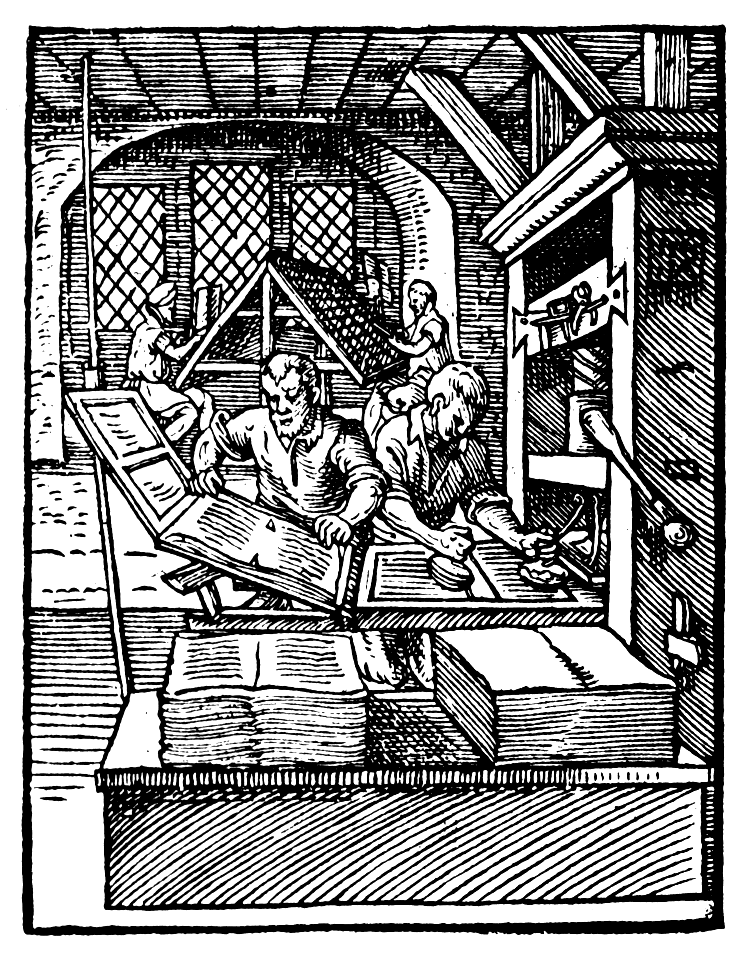
\includegraphics[width=0.8\textwidth]{fig/printer.png}
				\caption{Textsetzer im Jahre 1568 --- (Wikipedia) }
			\end{figure}
		\end{column}
	\end{columns}
\end{frame}

\begin{frame}
	\frametitle{Was ist Git? \hfill{} \footnotesize{FOSA}}
	\begin{columns}
		\begin{column}{5cm}
			\begin{figure}
				\centering
				
\includegraphics[width=0.8\textwidth]{fig/git_logo.pdf}
				\caption{Offizielles Git Logo}
			\end{figure}
			\footnotesize{
				\textbf{git}[\textipa{git}] - a bastard or fool
				\epigraph{\textit{"`I'm an egoistical bastard, and I name all 
				my projects after myself. First Linux, 
				now git."'}}{Linus Torvalds}
			}\normalsize
		\end{column}
		\begin{column}{5cm}
			\begin{block}{Überblick}
				\begin{itemize}
					\item Verwaltungssystem
					\item nicht linear
					\item dezentral
					\item sicher \& stabil
					\item FreeSoftware
					\item Plattformunabhängig
				\end{itemize}
			\end{block}
		\end{column}
	\end{columns}
\end{frame}

\begin{frame}
	\frametitle{Wozu ein Verwaltungstool?\hfill{} \footnotesize{FOSA}}
	\begin{columns}
		\begin{column}{5cm}
			\begin{figure}
				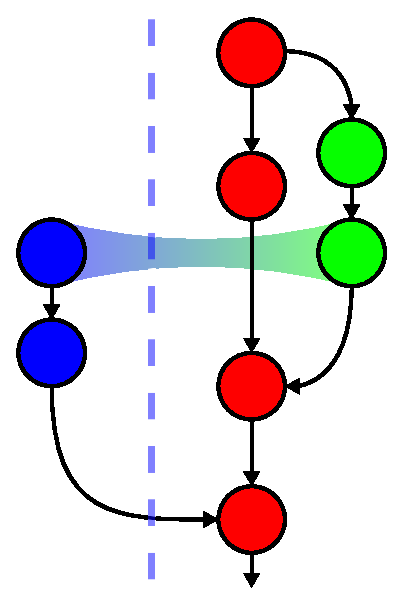
\includegraphics[scale=0.5]{fig/git_tree.eps}\\
				\textcolor{blue}{~~~~~~fork~~} -- 
				\textcolor{red}{~master~} -- 
				\textcolor{darkgreen}{~branch}
				\caption{Projetkbaum}
			\end{figure}
		\end{column}
		\begin{column}{5cm}
			\begin{block}{Fork, Master \& Branch}
				\begin{itemize}
					\item \textcolor{red}{Arbeiten an der FOSA}
					\item \textcolor{darkgreen}{Version FS13}
					\item \textcolor{darkgreen}{Korrekturen im FS13}
					\item \textcolor{blue}{Übernahme der Kopie und Erweiterungen}
		                        \item \textcolor{red}{Das Beste kommt zusammen für HS13}
				\end{itemize}
			\end{block}
		\end{column}
	\end{columns}
\end{frame}


\begin{frame}
	\frametitle{Github --- Social Coding \hfill{} \footnotesize{FOSA}}
	\begin{columns}
	        \begin{column}{5cm}
			\begin{figure}
				\centering
				
\includegraphics[scale=0.08]{fig/github_network.jpg}
			\end{figure}
				\vfill{}
			\begin{figure}
				\centering
				\includegraphics[scale=0.15]{fig/github_logo.eps}
				\caption{Github -- Soziales Netzwerk}
			\end{figure}
		\end{column}
		\begin{column}{5cm}
			\begin{block}{Was ist Github?}
		                \begin{itemize}
					\item Host für Repositories
					\item Private \& Enterprise
					\item Most Popular Host
				\end{itemize}
			\end{block}
			\begin{block}{Was ist speziell?}
				\begin{itemize}
					\item User im Zentrum
					\item Projekmanagement
					\item Git-Anbindung
					\item Simpel \& stabil
				\end{itemize}
			\end{block}
		\end{column}
	\end{columns}
\end{frame}

\end{document}
